\documentclass{article}
\usepackage[utf8]{inputenc}
\usepackage[T1]{fontenc}
\usepackage[english]{babel}
\setlength{\parindent}{0pt}
\usepackage{hyperref}
\hypersetup{
    colorlinks=true,
    linkcolor=blue,
    filecolor=magenta,      
    urlcolor=cyan}
\usepackage{graphicx}
\graphicspath{ {./pic/} }
\usepackage{multicol}
\usepackage{lscape}

\usepackage{fourier,amssymb,microtype,amsmath,gensymb}
\newcommand{\R}{\mathbb{R}}
\usepackage{mdframed,caption,xcolor}
\usepackage{tikz,tkz-euclide}

\title{Seminar 10. Incomplete Information in Dynamic Games}
\author{Xiaoguang Ling \\  \href{xiaoguang.ling@econ.uio.no}{xiaoguang.ling@econ.uio.no}}
\date{\today}

\begin{document}

\maketitle
 
%%%%%%%%%%%%%%%%%%%%%%%%%%%%%%%%%%%%%%%%%%%%%%%%%%%%%%%%%%%%%%%%%%%%%%%%%%%%%%%%%%%%%%%%%%%%%%
\section{Problem 1 - Screening and signaling}

Consider again the strategic situation described in Problem 1 of the exercise set for the nineth seminar, 

\begin{center}
Game $1$ \vspace{6pt}

$
\begin{array}{c|c|c|}
 & L & R \\
\hline
U & 0,0 & 4,2 \\
\hline
D & 2,6 & 0,8 \\
\hline
\end{array}
$
\end{center}

\begin{center}
Game $2$ \vspace{6pt}

$
\begin{array}{c|c|c|}
 & L & R \\
\hline
U' & 0,2 & 0,0 \\
\hline
D' & 2,0 & 2,2 \\
\hline
\end{array}
$
\end{center}

where only player 1 knows which game is being played, while player 2 thinks that the two games are \textbf{equally likely}.


\subsection*{(a) Screening} Assume now that \textbf{player 2 acts before player 1}, and that 2's choice can be observed by 1 before he makes his choice. Show that there is a unique subgame perfect Nash equilibrium. 

\begin{mdframed}[backgroundcolor=blue!20,linecolor=white]

Screening: Player \textbf{without} private information moves first $\Rightarrow$ there is nothing to infer (since player 1 knows everything, and player 2 has no chance to infer anything)

\begin{itemize}
\item Player 1 has private information: contingent strategy
\item Player 2 acts before player 1: can only choose between $L$ and $R$
\end{itemize}

\newpage

Extensive form:

\begin{center}
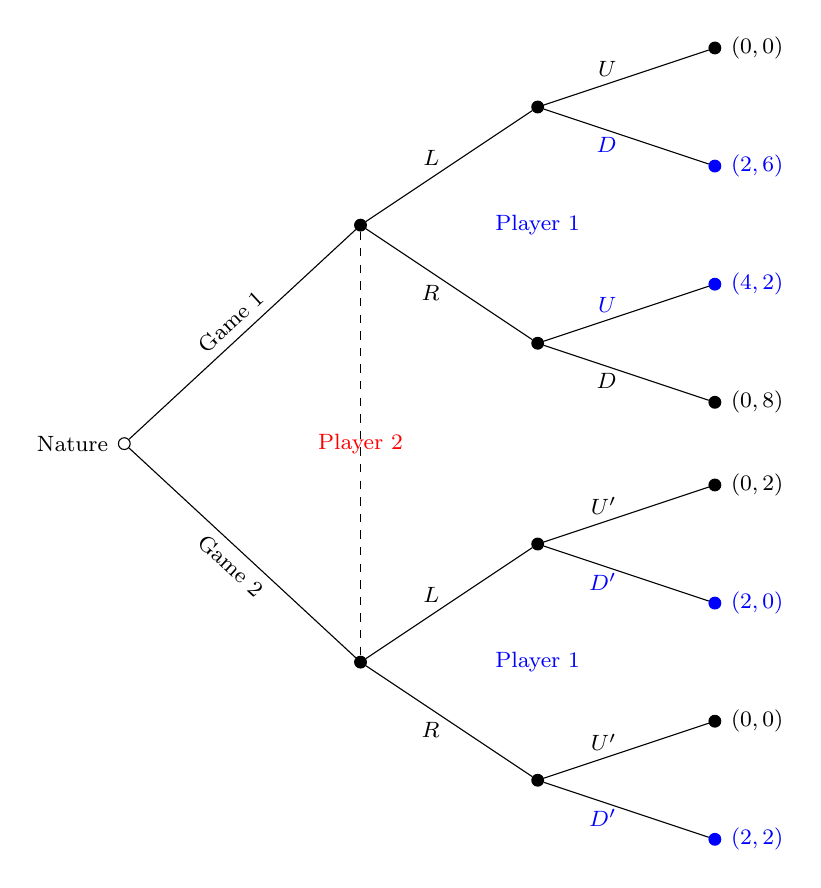
\begin{tikzpicture}[scale=1.5,font=\footnotesize]
\tikzset{
% Two node styles for game trees: solid and hollow
solid node/.style={circle,draw,inner sep=1.5,fill=black},
hollow node/.style={circle,draw,inner sep=1.5}
}
% Specify spacing for each level of the tree
\tikzstyle{level 1}=[level distance=20mm,sibling distance=37mm]
\tikzstyle{level 2}=[level distance=15mm,sibling distance=20mm]
\tikzstyle{level 3}=[level distance=15mm,sibling distance=10mm]
\tikzstyle arrowstyle=[scale=1]
\tikzstyle directed=[postaction={decorate,decoration={markings,
mark=at position .5 with {\arrow[arrowstyle]{stealth}}}}]

% The Tree
\node(0)[hollow node,label=left:{Nature}]{}[grow=east]
child{node(1)[solid node]{}
child{node(3)[solid node]{}
child{node[solid node,blue,label=right:{\textcolor{blue}{$(2,2)$}}]{}edge from parent node[left,blue,yshift=-3]{$D'$}}
child{node[solid node,label=right:{$(0,0)$}]{}edge from parent node[left,yshift=3]{$U'$}}
edge from parent node[left,yshift=-3]{$R$}}
child{node(4)[solid node]{}
child{node[solid node,blue,label=right:{\textcolor{blue}{$(2,0)$}}]{}edge from parent node[left,blue,yshift=-3]{$D'$}}
child{node[solid node,label=right:{$(0,2)$}]{}edge from parent node[left,yshift=3]{$U'$}}
edge from parent node[left,yshift=3]{$L$}
}
edge from parent node [midway, below, sloped] (TextNode) {Game 2}
}
child{node(2)[solid node]{}
child{node(5)[solid node]{}
child{node[solid node,label=right:{$(0,8)$}]{}edge from parent node[left,yshift=-3]{$D$}}
child{node[solid node,blue,label=right:{\textcolor{blue}{$(4,2)$}}]{}edge from parent node[left,blue,yshift=3]{$U$}}
edge from parent node[left,yshift=-3]{$R$}}
child{node(6)[solid node]{}
child{node[solid node,blue,label=right:{\textcolor{blue}{$(2,6)$}}]{}edge from parent node[left,blue,yshift=-3]{$D$}}
child{node[solid node,label=right:{$(0,0)$}]{}edge from parent node[left,yshift=3]{$U$}}
edge from parent node[left,yshift=3]{$L$}
}
edge from parent node [midway, above, sloped] (TextNode) {Game 1}
};
% information set
\draw [dashed] (2) -- (1) ;
% specify mover
\node at ($(1)!.5!(2)$) {\textcolor{red}{Player 2}};
\node at ($(5)!.5!(6)$) {\textcolor{blue}{Player 1}};
\node at ($(3)!.5!(4)$) {\textcolor{blue}{Player 1}};
\end{tikzpicture}
\end{center}

Player 1 acts contingently; Player 2 acts according to the expected payoff based on some belief $(\tfrac12,\tfrac12)$; 
\begin{itemize}
\item Use backward induction method to firstly determin how player 1 will react (in blue) and then calculate player 2's expected payoff.
\item We can also find when Game 2 is played, for player 1, $D'$ dominates $U'$
\end{itemize}

The contingent strategy for player 1 is easy to express, since there is no incomplete information.

\end{mdframed}

The strategy of player 1:
\begin{itemize}
\item If Game 1 is played:
\begin{itemize}
\item when player 2 chooses $L$, player 1 chooses $D$
\item when player 2 chooses $R$, player 1 chooses $U$
\end{itemize}
\item If Game 2 is played:
\begin{itemize}
\item when player 2 chooses $L$, player 1 chooses $D'$
\item when player 2 chooses $R$, player 1 chooses $D'$
\end{itemize}
\end{itemize}

For player 2:


$$E(U^2_L) = \tfrac12 \times 6 +\tfrac12 \times 0 = 3$$
$$E(U^2_R) = \tfrac12 \times 2 +\tfrac12 \times 2 = 2$$
$$\Rightarrow E(U^2_L) > E(U^2_R)$$

The strategy of player 2 is to choose $L$.

\medskip

Therefore there is only one SPNE:

\{(For player 1) In Game 1: $D$ after $L$, $U$ after $R$. In Game 2, $D'$ after $L$, $D'$ after $R$ ; (For player 2) $L$\}

\begin{mdframed}[backgroundcolor=blue!20,linecolor=white]
Compare the question with the \href{https://www.uio.no/studier/emner/sv/oekonomi/ECON4220/previous-exams/econ32_4220_2019h_sensorveiledning.pdf}{2019 exam problem 2(e)}. 

\medskip

Don't get tricked when the question says ``$U$ acts before $I$" but ``$U$ can choose between the four strategies $CC'$, $CE'$, 
$EC'$ and $EE'$ ''

\medskip

In the question, $U$'s strategy is like an agreement, which is passive and can only be activated by the choice of $I$; while only $I$ has contingent strategy.

\end{mdframed}

\subsection*{(b) Signaling} Assume now that player 1 acts before player 2, and that 1's choice can be observed by 2 before she makes her choice. Show that there is a unique separating perfect Bayesian equilibrium.

\bigskip

\begin{mdframed}[backgroundcolor=blue!20,linecolor=white]
Signaling: Player \textbf{with} private information moves first $\Rightarrow$ 
Player 2 can observe and infer the "type" of player 1.

\begin{itemize}
\item Both players have contingent strategy (Geir prefers not to distinguish player 2's contingent strategy in notation)
\item Player 2 observes $U/U'$ or $D/D'$ $\Rightarrow$ updates belief ($p\&q$) $\Rightarrow$ choose between $L$ and $R$
\end{itemize}

 where player 2's updated belief is:
\begin{itemize}
\item $Pr(\text{Game1} | U/U') = p$
\item $Pr(\text{Game1} | D/D') = q$
\end{itemize}



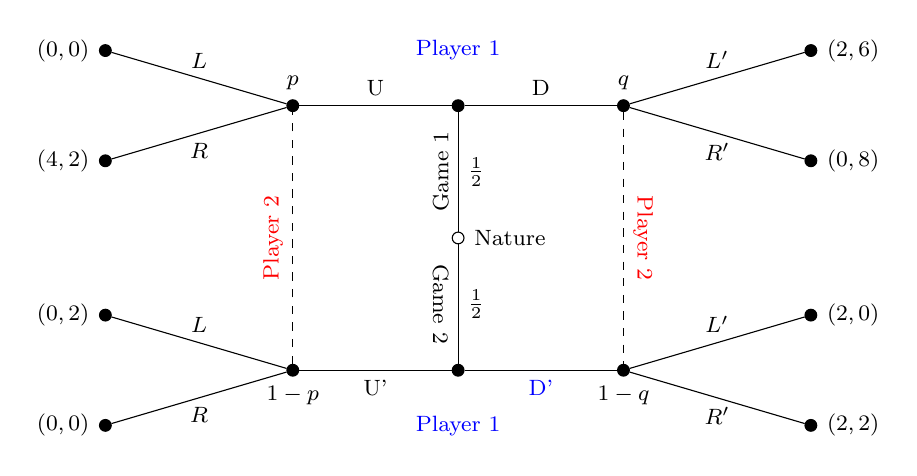
\begin{tikzpicture}[scale=1.4,font=\footnotesize]
\tikzset{
% Two node styles for game trees: solid and solid
solid node/.style={circle,draw,inner sep=1.5,fill=black},
hollow node/.style={circle,draw,inner sep=1.5}}
% Specify spacing for each level of the tree
\tikzstyle{level 1}=[level distance=12mm,sibling distance=25mm]
\tikzstyle{level 2}=[level distance=15mm,sibling distance=15mm]
\tikzstyle{level 3}=[level distance=17mm,sibling distance=10mm]
% The Tree
\node(0)[hollow node,label=right:{Nature}]{}
child[grow=up]{node[solid node,label=above:{
\begin{tabular}{c}
\textcolor{blue}{Player 1} \\ \\
\end{tabular}}] {}
child[grow=left]{node(1)[solid node,label=above:{$p$}]{}
child{node[solid node,label=left:{$(0,0)$}]{} edge from parent node [above]{$L$}}
child{node[solid node,label=left:{$(4,2)$}]{} edge from parent node [below]{$R$}}
edge from parent node [above]{U}}
child[grow=right]{node(3)[solid node,label=above:{$q$}]{}
child{node[solid node,label=right:{$(0,8)$}]{} edge from parent node [below]{$R'$}}
child{node[solid node,label=right:{$(2,6)$}]{} edge from parent node [above]{$L'$}}
edge from parent node [above]{D}
}
edge from parent node [right]{$\tfrac12$} node [midway, above, sloped] (TextNode){Game 1}
}
child[grow=down]{node[solid node,label=below:{\begin{tabular}{c}
\\ \textcolor{blue}{Player 1}
\end{tabular}}] {}
child[grow=left]{node(2)[solid node,label=below:{$1-p$}]{}
child{node[solid node,label=left:{$(0,2)$}]{} edge from parent node [above]{$L$}}
child{node[solid node,label=left:{$(0,0)$}]{} edge from parent node [below]{$R$}}
edge from parent node [below]{U'}
}
child[grow=right]{node(4)[solid node,label=below:{$1-q$}]{}
child{node[solid node,label=right:{$(2,2)$}]{} edge from parent node [below]{$R'$}}
child{node[solid node,label=right:{$(2,0)$}]{} edge from parent node [above]{$L'$}}
edge from parent node [below]{\textcolor{blue}{D'}}
}
edge from parent node [right]{$\tfrac12$} node[midway, below, sloped] (TextNode){Game 2}
};
% information set
\draw [dashed] (2) -- (1) node [midway, above, sloped, red] (TextNode) {Player 2};
\draw [dashed] (3) -- (4) node [midway, above, sloped, red] (TextNode) {Player 2};
\end{tikzpicture}

Note that for player 1, when Game 2 is played, $D'$ dominates $U'$. Therefore player 1 can 
only have 2 possible strategies: $UD'$ (if separating) and $DD'$(if pooling).

\medskip

The question wants you to show there is a unique separating PBE. So you only need to show $UD'$ can be part of a PBE.

\bigskip

\textbf{(1) Separating PBE}

\medskip

If player 2 believes $UD'$ is the strategy of player 2, then
$$p=1, q=0$$
and the BR of player 2 is $RR'$.

\medskip

\textbf{Will player 1 deviate from $U$ to $D$ if Game 1 is played? }No, if player 1
deviates to $D$, according to player 2's belief (player 2 believes Game 2 is played and thus chooses $R'$), the payoff is $(0,8)$, lower than $(4,2)$ if not deviate.

\medskip

This is therefore a unique separating PBN:

$$\{UD',RR',p=1,q=0\}$$

(don't forget the belief supporting the PBN)

\bigskip

\textbf{(2) Pooling PBE}

\medskip

There actually can also be a pooling PBE.

\medskip

If player 2 believes $DD'$ is the strategy of player 2, then
$$q=Pr(\text{Game 1})=\tfrac12$$

\medskip

You can apply the conclusion $q=Pr(\text{Game 1})$ in a pooling PBE directly, but this is acutally consistent with Bayes' rule:

\begin{align*}
Pr(\text{Game1} | D/D') &= \frac{Pr(D/D'|\text{Game1}) Pr(\text{Game1})}{Pr(D/D')} \\
&= \frac{1 \times \tfrac12}{1}
\end{align*}

Therefore, when observing $D/D'$, player 2's expected payoff is:

$$E[U^2_{L'}] = \tfrac12 \times 6+ \tfrac12 \times 0 = 3$$
$$E[U^2_{R'}] = \tfrac12 \times 8+ \tfrac12 \times 2 = 5$$

Player 2's BR is $R'$.

\medskip

\textbf{Will player 1 deviate from $D$ to $U$ if Game 1 is played?} It depends on what player 2 will do if the "surprise" shows up.

\medskip

If player 2 chooses $R$ after $U$, player 1 will deviate; if player 2 chooses $L$ after $U$, there is no incentive to deviate.

\medskip

Then under what condition will player 2 chooses $L$ after $U$? Expected payoff!

$$E[U^2_{L}] = p \times 0+ (1-p)\times 2 = 2(1-p)$$
$$E[U^2_{R}] = p \times 2+ \tfrac12 \times 0 = 2p$$

$$E[U^2_{L}] \ge E[U^2_{R}] \Rightarrow 2(1-p) \ge 2p \Rightarrow p \le \tfrac12$$

To support the pooling PBE, we must have $p \le \tfrac12$.
Note here since $U$ is not expected by player 2, we don't need to think about Bayes' rule.

\medskip

The pooling PBE is:

$$\{DD', LR', p \le \tfrac12, q = \tfrac12\}$$

\textbf{However, this PBE is not realistic}. Since player 2 knows clearly that if Game 2 is played, $U'$ will never be chosen by player 1. Therefore $1-p = 0, p =1 \ge \tfrac12$.

\medskip

We can say that the PBE here is consistent with the definition of PBE, but unrealistic. This is a defect of PBE. In exam you'll often be asked about which PBE (either pooling or separating) is unrealistic/unlikely to happen.

\medskip

The following is how to answer the question in exam:
\end{mdframed}


(1) Draw the extensive form first

\begin{mdframed}[backgroundcolor=yellow!20,linecolor=white]
Important. Be careful about the order of payoff, who is player 1 and who is player 2.
\end{mdframed}

From the extensive form we can see $D'$ dominates $U'$.
Therefore there can only be one separating PBE where player 1's strategy is $UD'$

(2) Denote the updated belief of player 2:
\begin{itemize}
\item $Pr(\text{Game1} | U/U') = p$
\item $Pr(\text{Game1} | D/D') = q$
\end{itemize}

For the separating PBE, $p=1,q=0$. The BR of player 2 is
$RR'$. Therefore the PBE is

$$\{UD',RR',p=1,q=0\}$$

\section{Problem 2 - Signaling pizza problem}

Consider the situation of Problem 1 of the eighth seminar, but assume now in addition that the pizza comes in 5
different sizes, each with $x$ slices, where $x \in \{4, 6, 8, 10, 12\}$. \textbf{Player 1 observes $x$}
before making her demand, while players 2 only observes player 1's demand, but not $x$, before
having to make his own demand. Before observing player 1's demand, player 2 thinks that the 5
different pizza sizes are equally likely, but he may infer something from her demand.
%
\subsection*{(a) Explain what a strategy is for player 1 in this game of incomplete information.} 
%
Player 1's strategy is contingent on the size of pizza ($x$), i.e. $s_1(x)$, 
where $x \in \{4, 6, 8, 10, 12\}$.

\subsection*{(b) Perfect Bayesian
equilibrium} Show that the following strategy for player 1 can be part of a perfect Bayesian
equilibrium: $s_1(4) = 2$, $s_1(6) = 3$, $s_1(8) = 4$, $s_1(10) = 5$, $s_1(12) = 11$. Specify
both player 2's strategy and player 2's beliefs. 
%

\begin{mdframed}[backgroundcolor=blue!20,linecolor=white]

The strategy can only be part of a separating PBE. In this case, player 2 believes
that player 1 sends signals by taking half the pizza, i.e. he thinks the size is $4,6,8,10,12$ once he observes player 1 asked for $2,3,4,5,11$.

\medskip 

Denote player 2's belief (probability on sizes $4, 6, 8, 10, 12$) as $\mu(x)$, and the BR of player 2 as $s_2^*$, we have:

\begin{center}
\begin{tabular}{|c|ccccc|c|}
\multicolumn{1}{c}{} & \multicolumn{6}{c}{Belief $\mu(x)$ for $x = \quad  \quad  \quad$}   \\
$s_1$ & $4,$ & $6,$ & $8,$ & $10$ & $12$ & $s_2^*$  \\   \cline{1-7} 
$2$ & $(1,$ & $0,$ & $0,$ & $0,$ & $0)$ & $2$ \\   
$3$ & $(0,$ & $1,$ & $0,$ & $0,$ & $0)$ & $3$ \\   
$4$ & $(0,$ & $0,$ & $1,$ & $0,$ & $0)$ & $4$ \\   
$5$ & $(0,$ & $0,$ & $0,$ & $1,$ & $0)$ & $5$ \\   
$11$& $(0,$ & $0,$ & $0,$ & $0,$ & $1)$ & $1$ \\   
\hline 
\end{tabular}
\end{center}
\textbf{Note that the belief above is required by Bayes' rule.}

\medskip

What if player 1 surprisingly asked for, for example, 6 slices? As long as the payoff is lower than PBE result, there is no deviation. The following belief can make sure so:

\begin{center}
\begin{tabular}{|c|ccccc|c|}
\multicolumn{1}{c}{} & \multicolumn{6}{c}{Belief $\mu(x)$ for $x = \quad  \quad  \quad$}  \\
$s_1$ & $4,$ & $6,$ & $8,$ & $10$ & $12$ & $s_2^*$  \\   \cline{1-7}
$0$ & $(1,$ & $0,$ & $0,$ & $0,$ & $0)$ & $4$ \\   
$1$ & $(1,$ & $0,$ & $0,$ & $0,$ & $0)$ & $3$ \\    \hline 
\textcolor{blue}{$2$} & $(1,$ & $0,$ & $0,$ & $0,$ & $0)$ & $2$ \\   
\textcolor{blue}{$3$} & $(0,$ & $1,$ & $0,$ & $0,$ & $0)$ & $3$ \\   
\textcolor{blue}{$4$} & $(0,$ & $0,$ & $1,$ & $0,$ & $0)$ & $4$ \\   
\textcolor{blue}{$5$} & $(0,$ & $0,$ & $0,$ & $1,$ & $0)$ & $5$ \\  \hline  
$6$ & $(0,$ & $0,$ & $0,$ & $0,$ & $1)$ & $6$ \\   
$7$ & $(0,$ & $0,$ & $0,$ & $0,$ & $1)$ & $5$ \\   
$8$ & $(0,$ & $0,$ & $0,$ & $0,$ & $1)$ & $4$ \\   
$9$ & $(0,$ & $0,$ & $0,$ & $0,$ & $1)$ & $3$ \\   
$10$& $(0,$ & $0,$ & $0,$ & $0,$ & $1)$ & $2$ \\  \hline    
\textcolor{blue}{$11$}& $(0,$ & $0,$ & $0,$ & $0,$ & $1)$ & $1$ \\ \hline 
$12$ & $(0,$ & $0,$ & $0,$ & $0,$ & $1)$ & $\ge 1$ \\   
\end{tabular}
\end{center}

Note that the belief for strategies in black is \textbf{NOT} required by Bayes' rule.

\medskip

For example, if the size $x=10$, on the equilibrium path, player 1 should ask for
5. But if player 1 surprisingly asks for 6, according to player 2's belief (player 2 
believes the size is 12), player 2 asks for 6 and the payoff is $(0,0)$. There is no incentive to deviate.
\end{mdframed}

\subsection*{(c) Are there other perfect Bayesian equilibria in this game?} %

\begin{mdframed}[backgroundcolor=blue!20,linecolor=white]

Here is another example of PBE: player 2 thinks that player 1 sends signal by taking $x-1$ slices of pizza; if player 2 thinks player 1 surprisingly took the whole pizza, he will ruin the pizza to punish player 1. There is no incentive to deviate.
\begin{center}
\begin{tabular}{|c|ccccc|c|}
\multicolumn{1}{c}{} & \multicolumn{6}{c}{$\mu(x)$ for $x =$}  \\
$s_1$ & $4,$ & $6,$ & $8,$ & $10$ & $12$ & $s_2^*$  \\   \cline{1-7}
$0$ & $(1,$ & $0,$ & $0,$ & $0,$ & $0)$ & $4$ \\   
$1$ & $(1,$ & $0,$ & $0,$ & $0,$ & $0)$ & $3$ \\    
$2$ & $(1,$ & $0,$ & $0,$ & $0,$ & $0)$ & $2$ \\   
\textcolor{blue}{$3$} & $(1,$ & $0,$ & $0,$ & $0,$ & $0)$ & $1$ \\  \hline  
$4$ & $(1,$ & $0,$ & $0,$ & $0,$ & $0)$ & $\ge 1$ \\   
\textcolor{blue}{$5$} & $(0,$ & $1,$ & $0,$ & $0,$ & $0)$ & $1$ \\  \hline  
$6$ & $(0,$ & $1,$ & $0,$ & $0,$ & $0)$ & $\ge 1$ \\   
\textcolor{blue}{$7$} & $(0,$ & $0,$ & $1,$ & $0,$ & $0)$ & $1$ \\   \hline 
$8$ & $(0,$ & $0,$ & $1,$ & $0,$ & $0)$ & $\ge 1$ \\   
\textcolor{blue}{$9$} & $(0,$ & $0,$ & $0,$ & $1,$ & $0)$ & $1$ \\  \hline  
$10$& $(0,$ & $0,$ & $0,$ & $1,$ & $0)$ & $\ge 1$ \\      
\textcolor{blue}{$11$}& $(0,$ & $0,$ & $0,$ & $0,$ & $1)$ & $1$ \\ \hline 
$12$ & $(0,$ & $0,$ & $0,$ & $0,$ & $1)$ & $\ge 1$ \\   
\end{tabular}
\end{center} 

\end{mdframed}

\bigskip

\section{Problem 3 - Challenging an incumbent}

Consider a market where there is an incumbent firm and a challenger. The challenger is
\textit{strong} with probability $\tfrac12$ and \textit{weak} with probability $\tfrac12$; it knows its type, but the incumbent
does not. The challenger may either \textit{prepare} itself for battle or remain \textit{unprepared}. The
incumbent observes the challenger's preparedness, but not its type, and chooses whether to
\textit{fight} ($F$) or \textit{acquiesce} ($A$). The extensive form and the payoffs are given by the following
figure. The challenger's payoff is listed first, the incumbent's second.


\bigskip

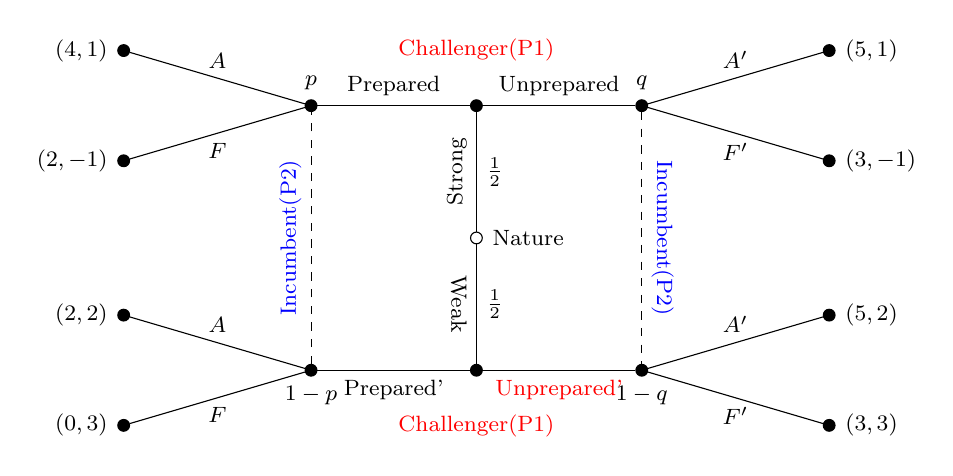
\begin{tikzpicture}[scale=1.4,font=\footnotesize]
\tikzset{
% Two node styles for game trees: solid and solid
solid node/.style={circle,draw,inner sep=1.5,fill=black},
hollow node/.style={circle,draw,inner sep=1.5}}
% Specify spacing for each level of the tree
\tikzstyle{level 1}=[level distance=12mm,sibling distance=25mm]
\tikzstyle{level 2}=[level distance=15mm,sibling distance=15mm]
\tikzstyle{level 3}=[level distance=17mm,sibling distance=10mm]
% The Tree
\node(0)[hollow node,label=right:{Nature}]{}
child[grow=up]{node[solid node,label=above:{
\begin{tabular}{c}
\textcolor{red}{Challenger(P1)} \\ \\
\end{tabular}}] {}
child[grow=left]{node(1)[solid node,label=above:{$p$}]{}
child{node[solid node,label=left:{$(4,1)$}]{} edge from parent node [above]{$A$}}
child{node[solid node,label=left:{$(2,-1)$}]{} edge from parent node [below]{$F$}}
edge from parent node [above]{Prepared}}
child[grow=right]{node(3)[solid node,label=above:{$q$}]{}
child{node[solid node,label=right:{$(3,-1)$}]{} edge from parent node [below]{$F'$}}
child{node[solid node,label=right:{$(5,1)$}]{} edge from parent node [above]{$A'$}}
edge from parent node [above]{Unprepared}
}
edge from parent node [right]{$\tfrac12$} node [midway, above, sloped] (TextNode){Strong}
}
child[grow=down]{node[solid node,label=below:{\begin{tabular}{c}
\\ \textcolor{red}{Challenger(P1)}
\end{tabular}}] {}
child[grow=left]{node(2)[solid node,label=below:{$1-p$}]{}
child{node[solid node,label=left:{$(2,2)$}]{} edge from parent node [above]{$A$}}
child{node[solid node,label=left:{$(0,3)$}]{} edge from parent node [below]{$F$}}
edge from parent node [below]{Prepared'}
}
child[grow=right]{node(4)[solid node,label=below:{$1-q$}]{}
child{node[solid node,label=right:{$(3,3)$}]{} edge from parent node [below]{$F'$}}
child{node[solid node,label=right:{$(5,2)$}]{} edge from parent node [above]{$A'$}}
edge from parent node [below]{\textcolor{red}{Unprepared'}}
}
edge from parent node [right]{$\tfrac12$} node[midway, below, sloped] (TextNode){Weak}
};
% information set
\draw [dashed] (2) -- (1) node [midway, above, sloped, blue] (TextNode) {Incumbent(P2)};
\draw [dashed] (3) -- (4) node [midway, above, sloped, blue] (TextNode) {Incumbent(P2)};
\end{tikzpicture}

\medskip

\subsection*{(a) What are the (pure) strategies for the challenger?} 


The challenger's strategy set: $\{PP', PU', UP', UU'\}$.

\begin{mdframed}[backgroundcolor=blue!20,linecolor=white]
Contingent on the type. For example, $PU'$ means "Prepared if I'm strong, Unprepared if I'm weak".
\end{mdframed}

\subsection*{(b) Why is there no perfect Bayesian equilibrium where the weak challenger chooses
\textit{Prepared}$'$ ? }

Prepared$'$ is dominated by Unprepared$'$.
It is always better for the weak challenger to choose $U'$, independently of
what the incumbent does.

\begin{mdframed}[backgroundcolor=blue!20,linecolor=white]
Is {Prepared} dominated by {Unprepared} (for strong challenger)?
No! If the Incumbent has (contingent) strategy $AF'$, Prepared has better payoff.
\end{mdframed}

\subsection*{(c) Separating}Show that there is a perfect Bayesian equilibrium where the strong challenger chooses
\textit{Prepared} and the weak challenger chooses \textit{Unprepared}$'$. 

Denote the updated belief of player 2:
\begin{itemize}
\item $Pr(\text{Strong} | P/P') = p$
\item $Pr(\text{Weak} | U/U') = q$
\end{itemize}

For the separating PBE, $p=1,q=0$. The BR of the incumbent is
$AF'$. Therefore the PBE is

$$\{PU',AF',p=1,q=0\}$$

\begin{mdframed}[backgroundcolor=blue!20,linecolor=white]
Will the challenger deviate?
\end{mdframed}

\subsection*{(d) Pooling}Show that there is a perfect Bayesian equilibrium where the strong challenger chooses
\textit{Unprepared} and the weak challenger chooses \textit{Unprepared}$'$. What do we call such an
equilibrium? 


For the pooling PBE, $q=Pr(\text{Strong})= \tfrac12$ according to Bayes' rule.

$$E[U^I_{A'}] = \tfrac12 \times 1+ \tfrac12 \times 2 =1.5$$
$$E[U^I_{F'}] = \tfrac12  \times (-1)+ \tfrac12 \times 3 = 1 $$

The BR of player 2 is $A'$. For a strong challenger, choosing U will lead to payoff result $(5,1)$. Higher than deviating to P no matter what the incumbent does. There can be 2 pooling PBE:

\medskip

(1) When the challenger surprisingly chooses $P/P'$, the incumbent chooses $A$:

$$E[U^I_{A}] = p \times 1+ (1-p)\times 2 = p + 2(1-p) = 2 - p$$
$$E[U^I_{F}] = p \times (-1)+ \tfrac12 \times 3 = -p + 3(1-p) = 3 - 4p$$

$$E[U^I_{A}] \ge E[U^I_{F}] \Rightarrow 2-p \ge 3-4p \Rightarrow p \ge \tfrac13$$

The PBE is

$$\{UU',AA',p \ge \tfrac13, q=\tfrac12\}$$

\medskip

(2) When the challenger surprisingly chooses $P/P'$, the incumbent chooses $F$:

$$E[U^I_{A}] \le E[U^I_{F}] \Rightarrow 2-p \le 3-4p \Rightarrow p \le \tfrac13$$

The PBE is

$$\{UU',FA',p \le \tfrac13, q=\tfrac12\}$$

\begin{mdframed}[backgroundcolor=blue!20,linecolor=white]
Which pooling PBE is more likely to happen? Why?
\end{mdframed}

\end{document}
